\begin{figure}[ht]
\centering
\subfigure[Moduł sprężystości objętościowej]{%
    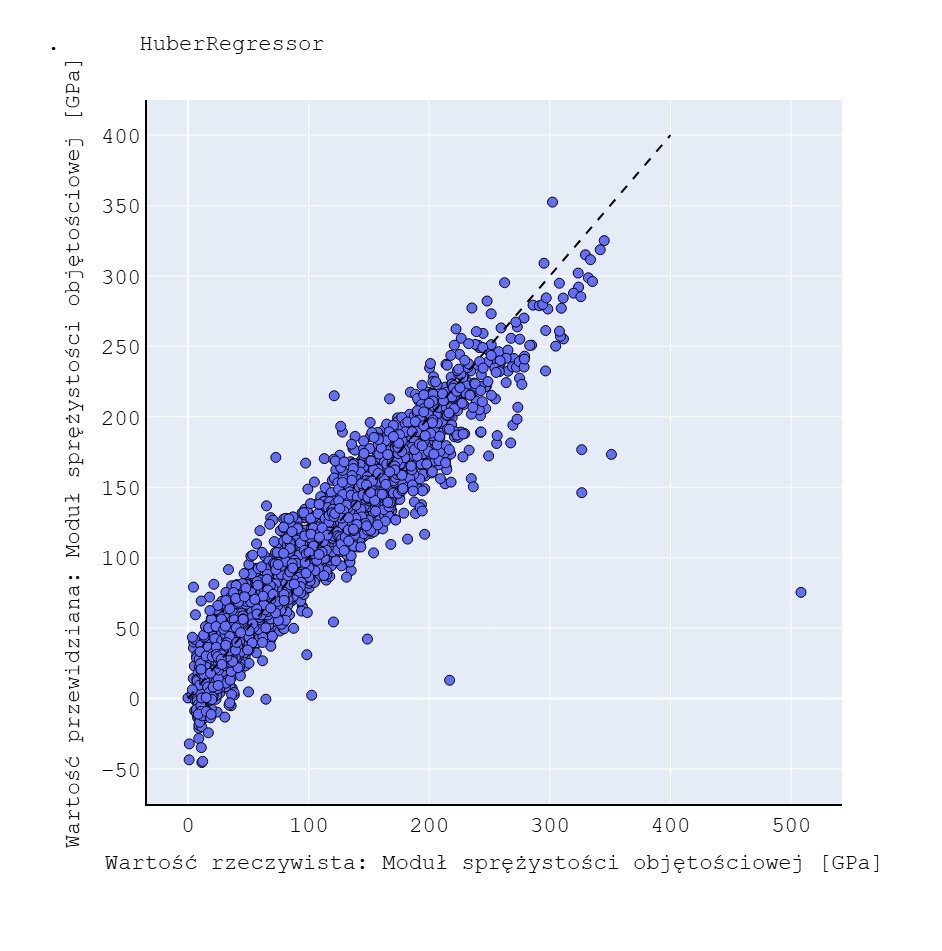
\includegraphics[width=0.48\textwidth]{images/figures/newplot (4).png}
}
\subfigure[Moduł sprężystości poprzecznej]{%
    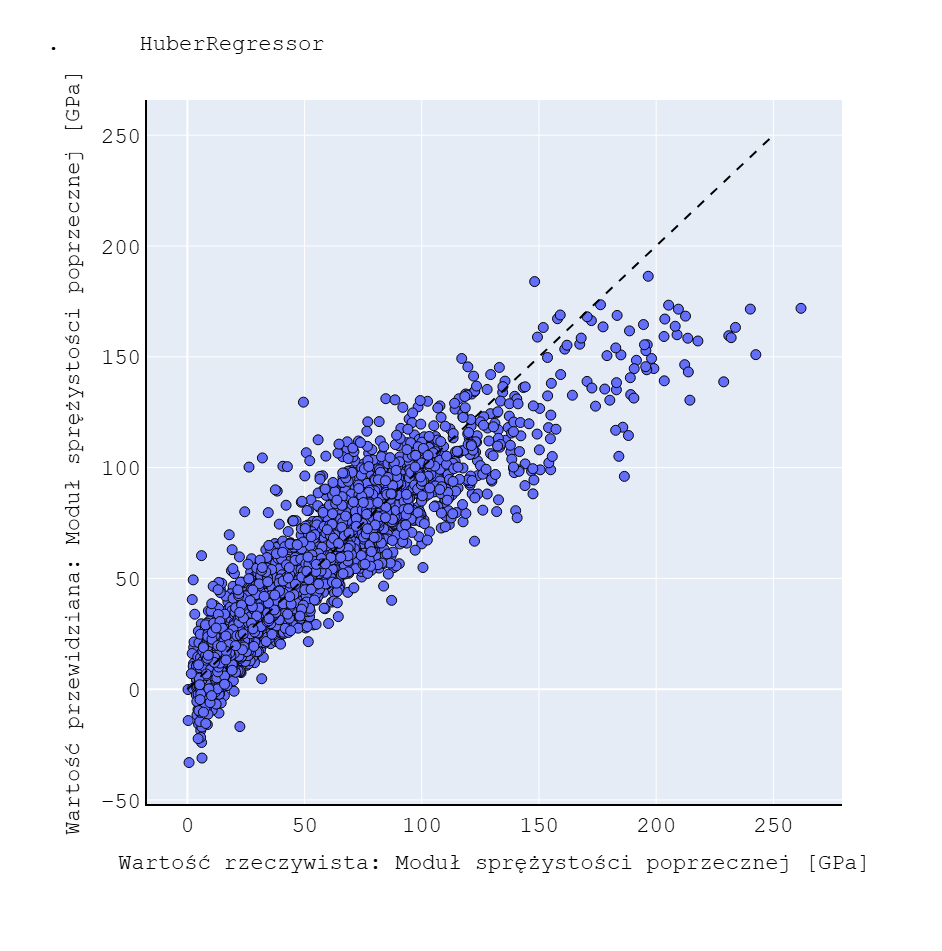
\includegraphics[width=0.48\textwidth]{images/figures/newplot (13).png}
}
\\
\subfigure[Współczynninik Anizotropii]{%
    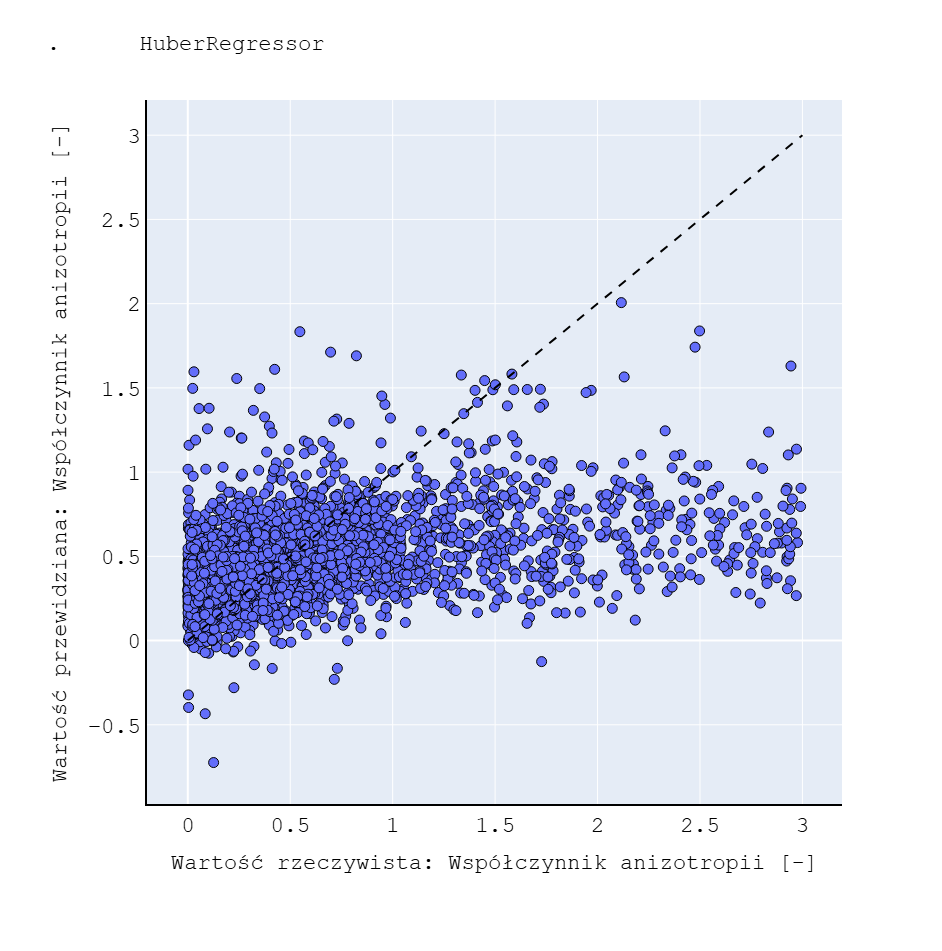
\includegraphics[width=0.48\textwidth]{images/figures/newplot (22).png}
}
\subfigure[Liczba Poisona]{%
    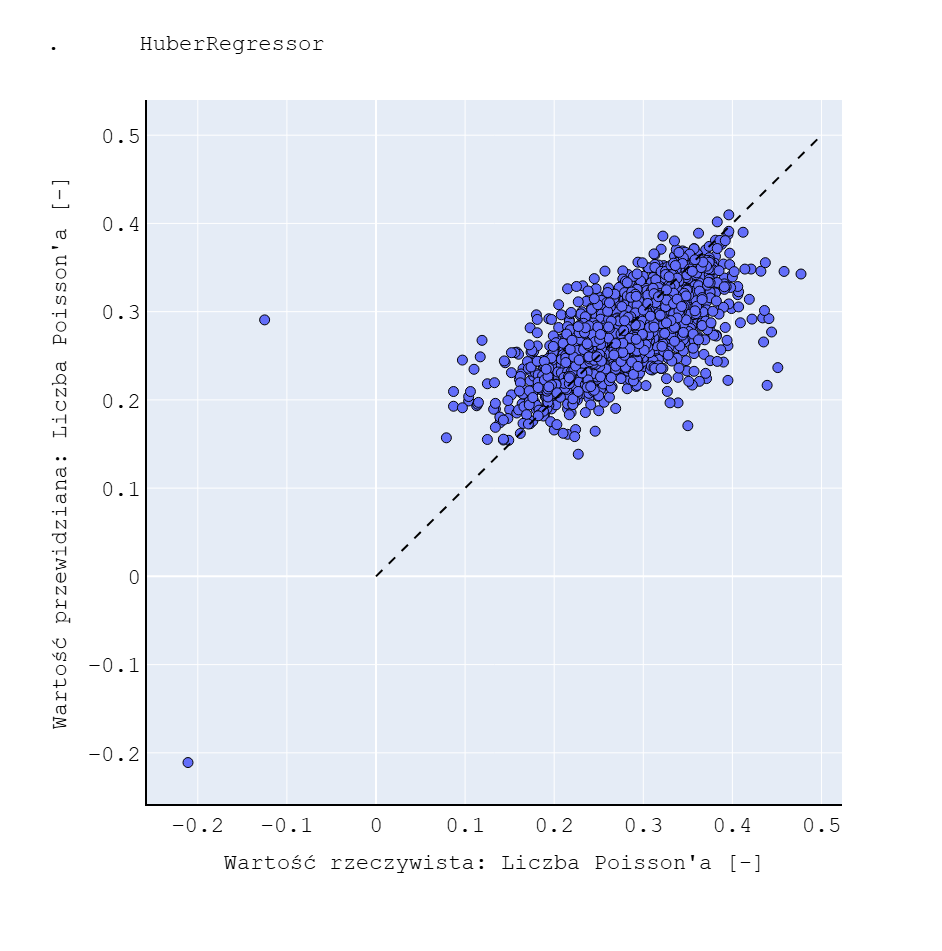
\includegraphics[width=0.48\textwidth]{images/figures/newplot (31).png}
}
\caption{Regresja Huber'a}
\end{figure}


podsumowanie liniowych

\clearpage